\documentclass{article} % For LaTeX2e
\usepackage{nips12submit_e,times}
%\documentstyle[nips12submit_09,times,art10]{article} % For LaTeX 2.09

\usepackage{amsmath,amssymb,amsthm,amsfonts,comment}
\usepackage{graphicx}\graphicspath{{figures/}}
\usepackage[small,labelfont=bf]{caption}
\usepackage[square]{natbib}
\usepackage{color}
\usepackage{subfigure}
\usepackage{epstopdf}
\usepackage{subfig}
\usepackage{dsfont}
\newlength{\subfigheight}
\setlength{\subfigheight}{1in}
\newcommand{\theHalgorithm}{\arabic{algorithm}}
\usepackage{multirow} 
\DeclareMathOperator*{\argmin}{arg\,min}
\DeclareMathOperator*{\argmax}{arg\,max}

%% our math environment
\def\[#1\]{\begin{align}#1\end{align}}

\newcommand{\defn}[1]{{\bf #1}}

\newcommand{\defas}{:=}
\newcommand{\given}{\mid}

\newcommand{\Naturals}{\mathbb{N}}
\newcommand{\Rationals}{\mathbb{Q}}
\newcommand{\Reals}{\mathbb{R}}
\newcommand{\cS}{\mathcal{S}}
\newcommand{\X}{\mathbf{X}}
\newcommand{\Y}{\mathbf{Y}}
\newcommand{\st}{\,:\,}
\newcommand{\RInts}{\mathcal{I}_\Rationals}
\newcommand{\YSets}{\mathcal{Y}_\Reals}
\newcommand{\grad}{\bigtriangledown}
\definecolor{LimeGreen}{rgb}{0.1,0.9,0.1}
\definecolor{Maroon}{rgb}{0.9,0.1,0.1}

%% our math environment
 
\newtheorem{thm}{Theorem}
\newtheorem{cor}[thm]{Corollary}
\newtheorem{lem}[thm]{Lemma}
%\newtheorem{definition}{Definition}

\title{Kernel Sparsity Boost: Nonparametric \\ Bayesian Network Structure Learning \\ Over Arbitrary Variable Types}

\author{
Rachel Hodos
Computational Biology and Mathematics, NYU
\texttt{hodos@cims.nyu.edu}
\Xnd
Wojciech Zaremba \\
Computer Science, NYU \\
\texttt{woj.zaremba@gmail.com} \\
\Xnd
David Sontag \\
Computer Science, NYU \\
\texttt{dsontag@cs.nyu.edu} \\
}
%
% Using \Xnd between authors leaves it to \LaTeX{} to determine where to break
% the lines. Using \XND forces a linebreak at that point. So, if \LaTeX{}
% puts 3 of 4 authors names on the first line, and the last on the second
% line, try using \XND instead of \Xnd before the third author name.

\newcommand{\fix}{\marginpar{FIX}}
\newcommand{\new}{\marginpar{NEW}}

%\nipsfinalcopy % Uncomment for camera-ready version

\begin{document}


\maketitle

\begin{abstract}

Most approaches in Bayesian network structure learning either require discrete variables or assume that relationships between continuous variables are linear.  Here we propose a novel scoring function which can handle discrete or continuous data directly, and which allows for arbitrary nonlinear relationships.  The scoring function is based on kernelized regression and the kernel conditional independence (KCI) test, \cite{zhang2012kernel}.  On synthetic data, we compare our approach to the MMHC algorithm with the KCI test incorporated.  We also show results on real data from three very different domains.

\end{abstract}


\section{Introduction}
It is well known that Bayesian network structure learning for general distributions is intractable \cite{chickering1996learning}. However, often for real data distributions, we are still able to recover the Bayesian network structure. This implies that real data distributions have some special properties, which can simplify the process of structure recovery.  This  process is almost always based on computing local statistics, and then reasoning about global structure \cite{jaakkola2010learning, tsamardinos2006max}. 

Examples of local statistics are measures of the model complexity (e.g. number of parameters in case of BIC\cite{schwarz1978estimating}), and conditional independence tests e.g. based on mutual information.  We focus in this work on how to best measure dependency between nodes in empirical CPDs from Bayesian network. We are mainly interest in developing techniques applicable to discovery of structure in gene expression data. This implies that each random variable can either 1) take many values (when expression values are discretized), or 2) have continuous values. The first case poses challenges if one wants to estimate conditional distributions in order to perform CI tests, a.k.a the curse of dimensionality.  The second case also makes conditioning difficult- how should one properly condition on a continuous variable?  One solution is perform linear regression on the conditioning variable (this is the approach taken by partial correlation), however, we would not like to restrict ourselves to linear relationships.  Furthermore, an property of the vast majority of gene expression datasets is that there are much fewer samples than there are variables, e.g. 20000 variables, and 100 samples.   We focus our attention on addressing Bayesian network structure learning
in such a regime. 

Our main contribution is in designing efficient dependency test for Bayesian networks. It is kernelized conditional independence (KCI) with kernels sensitive to the particular types of dependence relations present in our domain of interest. We show that kernelized partial correlation with proper kernel in ``gene expression'' regime is almost always better than any other previously considered dependency test. 


\section{Related work}

\subsection{Scoring Functions}
There has been extensive research in the area of scoring functions for Bayesian network structure learning. An appropriate scoring function is very important, e.g. if one simply maximized the likelihood, one would almost always recover the complete graph structure (the intuition is that a finite sample of two variables, even if independent, will almost always appear at least a little bit dependent).  Hence regularization is crucial.  There are two general types of regularization terms:(1) based purely on model complexity, and more recently (2) data-dependent regularization terms \cite{brenner2013sparsityboost}.

To the first group belongs one of the most widely used scoring functions, which is Bayesian Information Criterion (BIC) \cite{schwarz1978estimating}.  Another popular score is the Bayesian Dirichlet score, (BDe), There are couple of others like Hannan–Quinn information criterion (HQC) \cite{hannan1979determination},
or Bayesian model comparison (BMC). A major drawback of scoring functions based purely on model complexity is that they have constant power regardless of the amount of data.  Hence even if there is strong evidence, e.g. that an edge should not be in the graph, such scoring functions won't take this into account.


\begin{comment}
Variety of such scoring functions calculate dependency between nodes conditioned on potential parents \cite{de2006scoring}. Usual measures of dependency are based on mutual information, conditional independence test, or are fully Bayesian. Fully Bayesian methods assume probability distribution over CPDs of independent variables, and dependent variables.

We should discuss:
\begin{itemize}
\item LL (Log-likelihood) (1912-22)
\item MDL/BIC (Minimum description length/Bayesian Information Criterion) (1978)
\item AIC (Bkaike Information Criterion) (1974)
\item NML (Normalized Minimum Likelihood) (2008)
\item MIT (Mutual Information Tests) (2006)
\end{itemize}
Use in Bayesian networks \cite{schafer2005empirical}

Existing independence tests:
\begin{itemize}
\item Pearson's $\chi$-squared.  The problem is the null hypothesis is independence, but independence is what we're trying to show.
\item \cite{bergsma2011nonparametric} applied a "partial-copula transform" to perform a non-parametric test of conditional independence.
\end{itemize}

Independence tests used in Bayesian networks
\begin{itemize}
\item \cite{schafer2005empirical} Here they learn a Gaussian Graphical Model (GGM) using estimates of the partial correlation matrix. 
\item \cite{opgen2007correlation} Here they learn an approximate causal structure on gene expression based on full-order partial correlation (as an approximation to lower-order partial correlation that is called for theoretically for a Bayesian network).
\item \cite{tsamardinos2006max} MMHC algorithm.  They use a test based on what is called the $G^2$ statistic (asymptotically distributed as $chi^2$) and they also talk about a couple other independence tests that we may want to look into.
\end{itemize}

\cite{margaritis2003learning}
\end{comment}

\subsection{Learning Bayesian network structures with continuous variables}
The simplest and most widely used Bayesian network models over continuous variables are Gaussian Bayesian networks (GBNs), where each variable is sampled from a linear combination of its parents' states, plus some Gaussian noise.  \cite{geiger1994learning} present a principled scoring function to learn such a network.  This is the only score for learning continuous networks in the bnlearn package \cite{scutari2009learning}.  This model, however, restricts the local relationships to be linear, and hence a more general model is desirable in many settings.

One important technique for modeling non-Gaussian continuous BNs is kernel density estimation (KDE).  For example, \cite{john1995estimating} introduced the {\it Flexible Bayes} model, using KDE to enable the Naive Bayes classifier to use non-Gaussian continuous features.  \cite{perez2009bayesian} extends this framework to more generally structured classifiers beyond Naive Bayes.  Both of these methods assume that the conditioning variable is discrete, and hence conditioning is performed in the straightforward way.  Other techniques must be applied when the conditioning variables are continuous.  \cite{hofmann1996discovering} use KDE to model the CPDs by estimating the joint distribution over parents and child, and dividing by an estimate of the parents' distribution.  They performed a greedy hill-climbing procedure, optimizing cross-validated log-likelihood regularized by an edge penalty.  \cite{hansen2004nonparametric} describes a conditional KDE procedure that has the same flavor as the KCI test used in this work, where the conditional density is estimated by regressing on the conditioning variable and then using kernels to estimate the density over the residuals.  In all of these techniques, the choice of kernel width is key to getting a good estimate, and many techniques have been proposed to make such a choice.  \cite{john1995estimating} propose a heuristic kernel width $\sigma = \frac{1}{\sqrt n}$, i.e. the density estimation becomes more local as the number of data points increases.  Alternatively, \cite{holmes2012fast}, propose cross-validation of the log-likelihood.  Another issue with these techniques is that the nonparametric density estimates incur a computational cost at the time of classification, since all data points used for training must be stored in order to compute the likelihood of a new data point.  However there are ways to address this, e.g. \cite{gurwicz2004rapid} use splines to approximate and evaluate the densities much more efficiently.  One final kernel-based approach worth mentioning is that of \cite{bach2002learning}, where kernels are used to learn hybrid Bayesian networks (i.e. variables can be either continuous or discrete), where all variables are treated as Gaussian in feature space.  They demonstrate how one could use this approach within a greedy hill-climbing procedure, as well as in a constraint-based approach.

There are also many approaches that do not use kernels.  \cite{imoto2001estimation}, use nonlinear regression to estimate gene networks, and this is extended in \cite{imoto2003bayesian} to use non-parametric heteroscedastic regression.  \cite{ickstadt2010nonparametric} define what they call Nonparametric Bayesian Networks, where they assume the data are sampled from a mixture of Gaussian Graphical Models. \cite{elidan2007ideal} present a general method for speeding structure search for continuous variable networks with common parametric distributions. 

There is also some interesting work using copulas, e.g. {\bf just list the canonical paper introducing copula BNs}  \cite{hanea2006hybrid}, \cite{hanea2008mixed}, and \cite{hanea2010mining}, but these papers focus on statistical inference and parameter estimation.  In terms of model selection, \cite{elidan2010copula} uses a standard score-and-search approach using the BIC score.  \cite{bauer2012pair} extend the popular constraint-based PC algorithm to use a conditional independence test fitting for their model, using parametric estimation of conditional distributions based on vine copula models.  \cite{elidan2012lightning} and \cite{tenzer2013speedy} leverage a one-to-one relationship between Spearmen's rho correlation and the log-likelihood term for an edge addition (asymptotically true for tree-structured networks) in order to learn copula networks efficiently.  In the first paper, they use a heuristic to extend the method to non-tree structured networks.  In the second paper, they only considered tree-structured BNs, but allowed each copula to have a different parameteric form, whereas in the first paper all copulas were restricted to the same parametric family.  In both works they optimize using the BIC score. {\bf verify my description with Gal Elidan.}

We are proposing a method which uses continuous data but does not estimate the conditional distributions- i.e. we are decoupling the problem of structure learning with parameter learning.  The work of \cite{margaritis2005distribution} also falls into this category, although they take a constraint-based approach, applying the PC algorithm to continuous data via a non-parametric, discretization-based independence test.

\section{The Kernel Sparsity Boost Score (KSB)}
In the section we describe our new scoring function, but first, we introduce some notation.  For each $X_i \in \mathcal{X}$, let Pa$_G(X_i)$ denote the parents of $X_i$ in the DAG G.   Throughout the paper, capital letters will denote random variables, e.g. $X_i, Pa(X_i)$, and lower case letters will denote instantiations, e.g. $x_i^n$ and $pa^n(x_i)$.  The n superscript denotes the $n^{th}$ data point.   When the context is clear we will drop the subscript G.  Finally, let $G^*$ denote the true network.

Like most scoring functions for Bayesian network structure learning, our score decomposes into a sum of scores for each family, i.e. a variable and its candidate parents.  Hence the KSB score for G given dataset D can be written as \begin{equation} KSB(G;D) = \sum_{X_i \in \mathcal{X}} ksb(X_i, Pa_G(X_i); D), \end{equation} where $ksb$ are the family scores, defined as \begin{equation} ksb(X_i, Pa_G(X_i); D) = \sum_{n \in 1, \ldots, N} \left(\mathbf{w}^T\Phi(pa^n(x_i)) - x_i^n \right)^2 + \sum_{X_j \in Pa(X_i)} \max_{C \in \Omega{ij}} sb(X_i, X_j|C; D) \end{equation}  

The first term is the sum of squares of residuals after performing kernel ridge regression of $X_i$ onto its parents in G.  $\Phi$ is the feature mapping corresponding to the kernel used in the regression\footnote{We use a Gaussian kernel throughout the paper for both regression and kernel conditional independence tests.}.  Recall from ordinary least squares regresion that minimizing the sum of squares of the residuals is exactly equivalent to maximizing the likelihood of the data under the assumption that the expectation of $X_i$ is drawn from a linear model plus some Gaussian noise with constant variance $\sigma^2$.  In the same way, the term presented here corresponds to the likelihood of the data given the chosen weight vector w.  Note that we wouldn't want to choose w using ML estimation, since this can lead to over-fitting, especially in the case of $\Phi(Pa(X_i))$ being infinite dimensional, such as when using a Gaussian kernel.  Hence the first term is a likelihood term.  Hence we perform kernel ridge regression, which adds the regularization penalty $\lambda \| w\|^2$ to the objective, improving the generalizability of the learned model.  {\bf David says that the risk we are minimizing is log-loss.  I guess I'm not sure what this means.}

The second term is a data-dependent regularization term, called the "Sparsity Boost" term following the framework presented in \cite{brenner2013sparsityboost}.  The idea of this term is to search for conditional independencies between pairs of variables in $\mathcal{X}$, and when there is strong evidence, to boost the scores of any graph which does not contain the corresponding edge.  The original presentation in \cite{brenner2013sparsityboost} was only applicable to binary variables, whereas here present an approach that can handle arbitrary continuous or discrete variables. 

\section{Independence testing} 
{\bf Notation} 
For generality of our statements, we consider random variables $X, Y, Z$ defined in domains $\mathcal{X}, \mathcal{Y}, \mathcal{Z}$. Moreover,
we define kernels for each of those variables, and we denote them respectively by $k_{\mathcal{X}}, k_{\mathcal{Y}}, k_{\mathcal{Z}}$.


Independence tests decides on independence of random variables. More formally,
for a random variables $X, Y$ given $Z$, test decides on equality $P(X, Y| Z) = P(X | Z) P(Y | Z)$. 
Figure \ref{fig:ind} presents surface of $2$ dimensional independent 
random variables $X, Y$, and $Z = \varnothing$. Independence choses if samples $x \in X, y \in Y, z \in Z$, 
are coming from independence surface, or not. 
This problem can be casted as a classification problem, and we define
empirical loss for it as:
\begin{equation}
  \mathbb{E}_{x \in X, y \in Y, z \in Z, t \in \{\text{indepedent}, \text{depedent}\}} L(f((x, y)|z, t)
\end{equation}
Our initial task is to find $f$, which well predicts independence given our prior
knowledge on $X, Y, Z$. Such task is not easy as the manifold of independent
random variables is highly non-linear. We review several approaches, and 
settle on kernel independence tests, which gives superior performance on
samples drawn from Bayesian networks.


There are few issues, which such test has to address 
(1) account for prior over $X, Y, Z$ \ref{sec:prior}, (2) diminishing number of samples when
counting occurrences \ref{sec:curse}. We discuss this issues
in following sections. 


\begin{figure}[h]
\centering
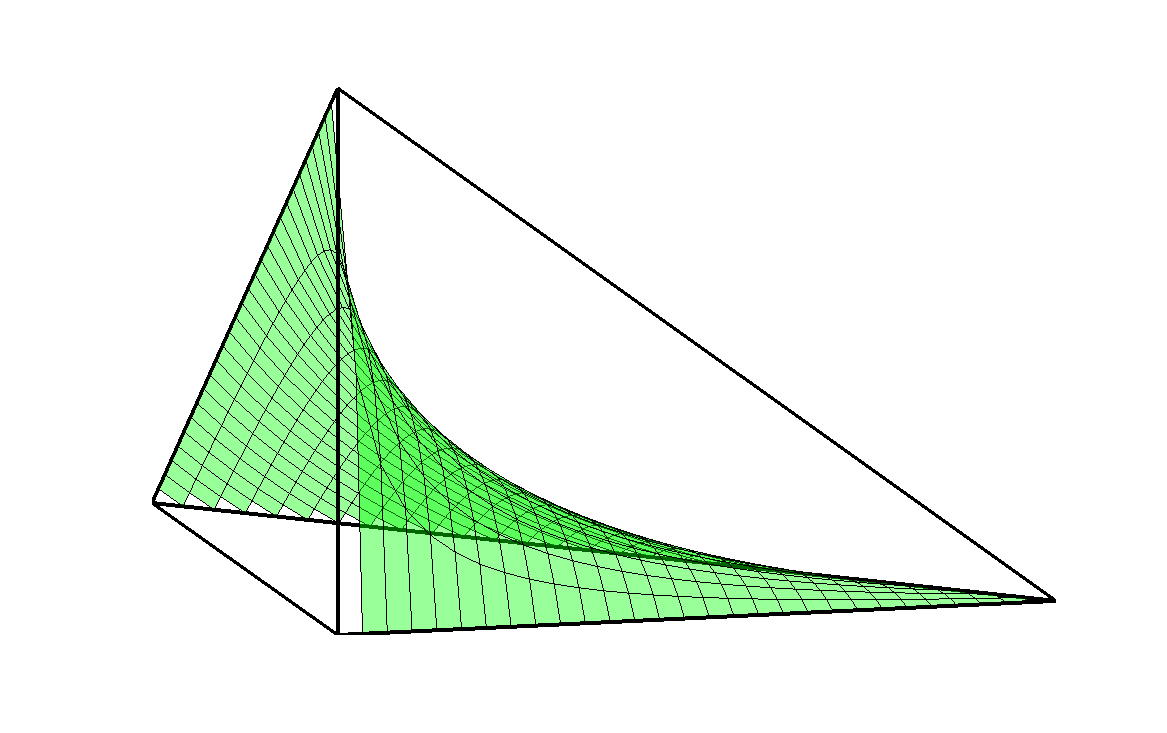
\includegraphics[width=0.35\linewidth]{img/independence_surface-eps-converted-to-crop.pdf}
\caption{The manifold of independence for binary distributions. The simplex represents all possible joint distributions over two binary variables parametrized with their marginal distributions. The simplex is formed by the constraint that marginal distributions must be positive and sum to one.  The manifold corresponds to the set (of measure zero) of independent distributions.}
\label{fig:ind}
\end{figure}

\subsection{Prior}\label{sec:prior}
Set $(X, Y, Z, t=\text{independent})$ has measure zero for uniform distribution over CPDs of $X, Y, Z$. For such distribution
best possible predictor $f$ would always predict ``dependence''. 
This shows that a prior coming from any natural parametrization
of CPDs would force $f$ to be constant. This indicate that, we should
employ better prior. We are interest in non-parametric priors over $(X, Y, Z)$.
Moreover, we would like our test to be consistent.


In gene expression data, random variables (gene expressions) can 
have arbitrary real values. Common practise is to quantize such values,
and count number of values in every bucket. However, this removes 
''smoothness`` prior over assignments. ``Smoothness'' prior means that
nearby values of random variables have a similar meaning. We can easily see
that common measure of dependency such as mutual information {\bf don't} have 
this property. 
\begin{align*}
  I(X;Y)=\sum_{a \in X}\sum_{b \in Y} p(a, b)\log{\frac{p(a, b)}{p(a)p(b)}}=I(\sigma_X(X), \sigma_Y(Y))
\end{align*}
$\sigma_X$ is a permutation over values of $X$, and $\sigma_Y$ is
a permutation over values of $Y$.


Another prevalent measure of dependency is correlation. This measure
has a notion of ``smoothness'' (it treats near by values similarly), but
it is not consistent. Moreover, empirical experiments show that zero value
of correlation often doesn't imply lack of dependency. We might want to 
enforce some level of smoothness (e.g. single differentiable vs infinitely 
differentiable functions). Correlation doesn't let us do that. 

Partial correlation, and its extension kernelized partial correlation (KCI), which are described 
in Sections \ref{sec:corr} both aforementioned smoothness properties.


\subsection{Curse of conditioning}\label{sec:curse}
Most of Bayesian structure learning methods first express data in conditional probabilities tables (CPT).
Next, various statistic are computed for such tables of probabilities. However, such step
for multi-label data might be already prohibitively expensive, as the size of tables grows
exponentially with number of labels per node. Moreover, CPTs cannot represent continuous
distributions. Usual engineering solution is to quantize data. This step is far from optimal,
as it decreases data resolution (removes information). 

High computational cost of methods based on CPTs statistic is not the only problem. 
CPTs based on moderate number of samples are very badly estimated. Xs the number
of entries in CPT grows exponentially, there might be some bins which stay empty. This might
be very dangerous for quality of independence test.

We aim for test, which avoids construction of CPTs, and can directly operate on continuous data.
We will see that KCI independence tests have such property (Table \ref{tab:compar}).

\subsection{Distance correlation}\label{sec:dist}
Distance correlation \cite{szekely2007measuring} is generalization of correlation, which is zero only for independent distributions.
Distance covariance, and distance correlations are defined as follow:
\begin{align*}
  &k_\mathcal{X} = XX^T \in \mathbb{R}^{n \times n},
  k_\mathcal{Y} = YY^T \in \mathbb{R}^{n \times n}\\
  &H = I - \frac{1}{n}11^T \\
  &\tilde{k}_\mathcal{X} = Hk_{\mathcal{X}}H, 
  \tilde{k}_\mathcal{Y} = Hk_{\mathcal{Y}}H \\
  &dCov^2(X, Y) = Tr(\tilde{k}_\mathcal{X}\tilde{k}_\mathcal{Y}) \\
  &dCorr^2(X, Y) = \frac{dCov^2(X, Y)}{\sqrt{\sum_{i=1}^nk_{\mathcal{X}}(x_i, x_i) \sum_{i=1}^nk_{\mathcal{Y}}(y_i, y_i)}} 
\end{align*}

Linear kernel used in above equations can be replaced with any kernel. $0 \leq dCorr^2(X, Y) \leq 1$, and $dCorr^2(X, Y) = 0$ iff X, Y are independent. 

\subsubsection{Partial correlation}\label{sec:corr}
The method of partial correlation measures the remaining correlation between two random variables $X, Y$ after regressing on $Z$ (a set of random 
variables on which we would like to condition).  The procedure computes the residuals $R_X, R_Y$ of each regression and then measures the correlation between the residuals. More formally:
\begin{align*}
  w_X &= \argmin_{w_X} ||x - w_X z||_{2} \\
  w_Y &= \argmin_{w_X} ||y - w_Y z||_{2} \\
  R_X &= x - w_X z \\
  R_Y &= y - w_Y z
\end{align*}
$x, y, z$ are samples of random variables $X, Y, Z$. When $Z = \varnothing$, then $R_X = x$, and $R_Y = y$, which
recovers correlation. Partial correlation is not able consistently decide
on independence of random variables. However, it has two desirable properties: (1) smoothness \ref{sec:prior} and (2)
acts on values instead of counts \ref{sec:curse}. Kernelized version of partial correlation for 
characteristic kernel recovers consistency.


\subsubsection{Kernelized partial correlation}\label{sec:kci}
Kernelized conditional independence (KCI) \cite{zhang2012kernel} is a ''marriage`` of concepts presented in 
previous Subsections \ref{sec:dist} and \ref{sec:corr}. KCI regresses $Z$ on $X, Y$ in kernel space with kernelized
ridge regression \cite{saunders1998ridge}. Next,
it applies distance correlation to regressors. Such statistic has all desired properties (1) consistency, (2) smoothness, 
(3) value based conditioning Table \ref{tab:compar}. We advocate in this paper, that this dependency measure
is best suitable for Bayesian networks learning. 


\begin{table}[t]
\centering
\tiny
\begin{tabular}{rrrrr}
\hline
Measure & Consistent & Smooth prior & Controllable smooth & Value based\\
& & & prior & conditioning\\
\hline
Mutual information & $\color{LimeGreen} \checkmark $ & $\color{Maroon}\times$ & $\color{Maroon}\times$ &   $\color{Maroon}\times$ \\
Correlation & $\color{Maroon}\times$  & $\color{LimeGreen} \checkmark $ & $\color{Maroon}\times$ & $\color{Maroon}\times$ \\
Distance correlation & $\color{LimeGreen}\times$  & $\color{LimeGreen} \checkmark $ & $\color{Maroon}\times$ & $\color{Maroon}\times$ \\
Partial correlation & $\color{Maroon}\times$  & $\color{LimeGreen} \checkmark $ & $\color{Maroon}\times$ & $\color{LimeGreen}\checkmark$ \\
KCI for non-characteristic kernel & $\color{Maroon}\times$  & $\color{LimeGreen} \checkmark $ & $\color{LimeGreen}\times$ & $\color{LimeGreen}\checkmark$ \\
KCI for characteristic kernel & $\color{LimeGreen}\checkmark$  & $\color{LimeGreen} \checkmark $ & $\color{LimeGreen}\times$ & $\color{LimeGreen}\checkmark$ \\
\hline
\end{tabular}
\caption{Comparison of properties for various independence tests. Consistency means if test would give correct answer with infinite amount of data. Smooth prior (Section \ref{sec:prior}) indicates if tests treats ''near by`` values in similar way. Controllable smooth prior tells if we can vary what we consider to be smooth. Value based conditioning (Section \ref{sec:curse}) say if test can avoid constructing conditional probabilities tables, which are expensive, and badly estimable.}
  
\label{tab:compar}
\end{table}


\section{Experiments}


\subsection{Synthetic data experiments}

\subsubsection{ROC curves}
In order to evaluate the power of the KCI test in comparison with other conditional independence statistics, we generated synthetic continuous data from several toy Bayesian networks, and then computed each statistic, taking the strongest evidence for independence over various conditioning sets in the same way that is done in the SparsityBoost framework.  Let f be the function which computes a statistic of interest. Then for each pair $X_i$ and $X_j$ we compute:  \begin{eqnarray*} T_f(i,j) &:=& \min_{S \in \Omega_{ij} } f(X_i,X_j | S; D) \\ \Omega_{ij} &:=& \{ S \in \mathbf{X} / \{i,j\} : |S| \leq 2 \} \end{eqnarray*}  Taking the minimum over all sets in $\Omega_{ij}$ corresponds to taking the strongest evidence of independence over all conditioning sets (that we choose to consider), since it is enough to find one conditioning set which renders $X_i$ and $X_j$ independent in order to conclude that edge $\{i,j\}$ should not be present.  We treat f as a classifier by thresholding at various values throughout the range, and then evaluate the true and false positive rates (with respect to all pairs of variables in the network) in order to generate ROC curves.  Here we define positive to mean independence, hence the point (0,0) in the plots corresponds to a classifier which always claims dependence, and likewise (1,1) corresponds to a classifier which always claims independence.

The data are generated as continuous variables with random quadratic relationships plus Gaussian noise.  More precisely, source nodes are drawn from $N(0, 0.1)$, and then variable with parents is defined as $X_i = \sum_{X_j \in Pa(X_i)} \alpha_j X_j^2 + \beta_j X_j + \epsilon $ where $\alpha_j$ and $\beta_j$ are drawn randomly from $N(0, 1)$ with the added constraint that they have magnitude greater than 0.3, and $\epsilon$ is the noise component, drawn from $N(0, 0.05)$.  

\begin{figure}[h]
\centering
    \subfigure{
      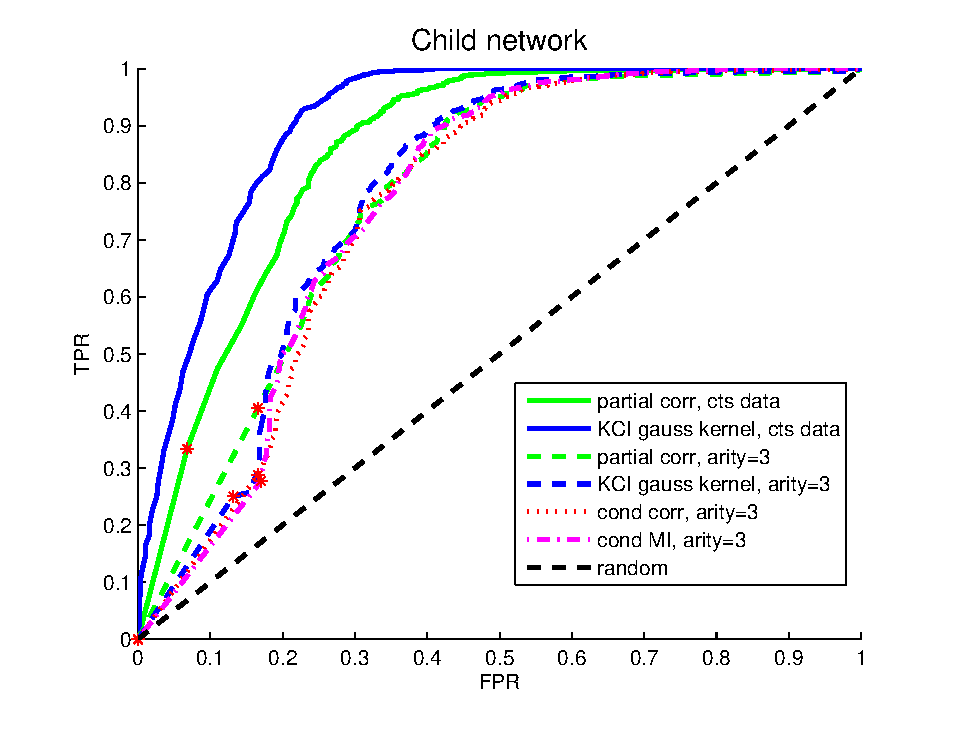
\includegraphics[width=0.45\linewidth]{img/child.eps} 
    }
    \quad
    \subfigure{
      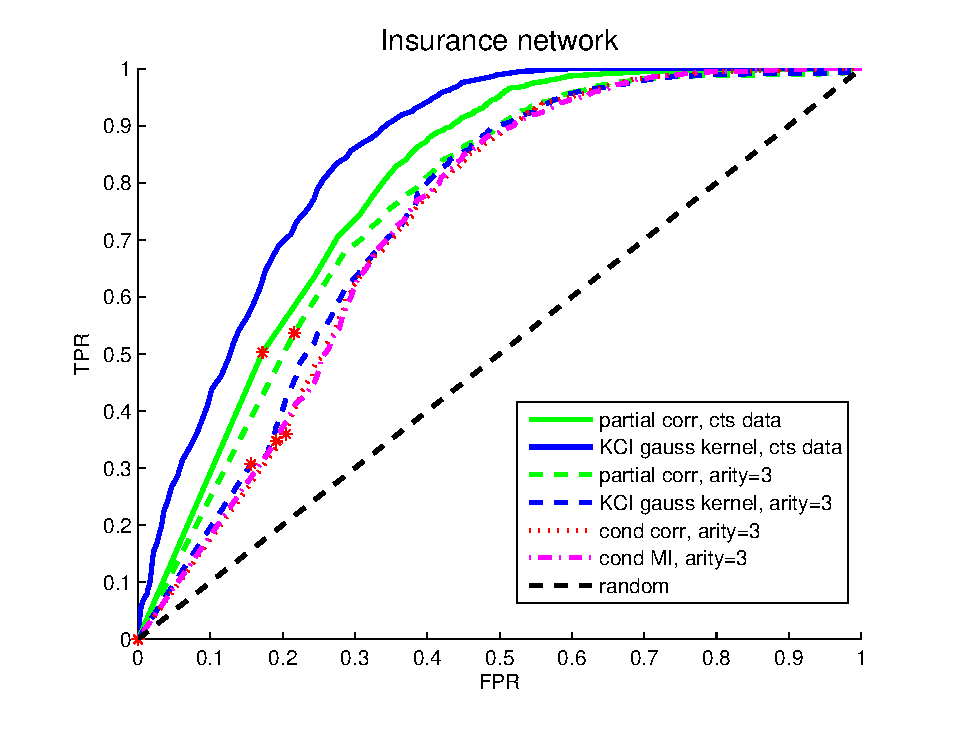
\includegraphics[width=0.45\linewidth]{img/insurance.eps} 
    }
\caption{ROC curves for classifying joint distributions generated from the ``child'' network structure (left) and ``insurance'' network structure (right).  All calculations were performed using N=100 data points, and each curve corresponds to an average over 20 repetitions (independent data samples).  Each variable is sampled from a random quadratic function of its parents values, plus Gaussian noise, as described in the text.  The solid curves correspond to classification using the original, continuous data, whereas the dashed curves were generated using data that were discretized into 3 uniformly-spaced bins for each variable.  The red asterisk on each curve corresponds to a threshold value of 1e-3 (the smallest one greater than zero tested).  Hence one can see that even though partial correlation using continuous data performs better than the classifiers that use discrete data, it has a high FPR even with an extremely small threshold, reflecting the fact that correlation is not consistent, i.e. a distribution with zero correlation could still be dependent.}
\label{fig:ROC}
\end{figure}

\subsubsection{Structure recovery}
We generated continuous synthetic data from three toy Bayesian networks, where each variable follows a random quadratic relationship with each of its parents, as described in the above section.  We then compared several algorithms' ability to recover the structure from which the synthetic data were generated (up to the Markov equivalence class).  We used three baselines for comparison.  The first is the MAP solution of the BIC score.  This of course requires discretization.  The results shown use four uniformly-spaced bins.  We also did some experiments using only three bins, and also tried quantile bin spacing (i.e. bins chosen so that marginals are uniform), and found that four uniformly-spaced bins generally performed better.  The MAP solution for both the BIC score and our novel score is found using the integer linear programming approach introduced in \cite{jaakkola2010learning}.  We use the GOBNILP 1.3 implementation \cite{cussens2012bayesian}, built upon the SCIP framework \cite{achterberg2009scip}.  The second baseline is the Max-Min Hill Climbing (MMHC) procedure \cite{tsamardinos2006max}, using KCI for the conditional independence test.  The third baseline is learning a simple linear Gaussian Bayesian network (GBN), i.e. assuming that each variable is a linear combination of its parents plus some Gaussian noise, i.e. $X_i =  \sum_{X_j \in Pa(X_i)} \beta_j X_j + \epsilon,$ where $\epsilon$ is $N(0, \sigma^2)$.  

\begin{table}[h]
\centering
\begin{tabular}{|c|c|c|c|l|}
\hline
Network Name & \# of nodes & \# of edges & max in-degree & Reference                         \\ \hline
Asia         & 8           & 8           & 2             & \cite{lauritzen1988local}        \\ \hline
Child        & 20          & 25          & 2             & \cite{spiegelhalter1992learning} \\ \hline
Insurance    & 27          & 52          & 3             & \cite{binder1997adaptive}        \\ \hline
\end{tabular}
\caption{Network structures used for synthetic data experiments.}
\label{networks}
\end{table}

The networks used are presented in Table \ref{networks}. For each network structure, we performed the following experiment.  For each value of $N$, the number of observations, we generated 10 random networks, i.e. parameter sets $(\vec{\alpha}, \vec{\beta})_k, k \in 1, \ldots, 10$.  For each of these networks, we sampled 3 independent datasets, each with $N$ data points.  We then threw out any observations where any of the variables were outside of the median $\pm$ three standard deviations.  The data were then normalized (to have mean 0, standard deviation 1), and discretized if necessary, then fed into each structure learning algorithm.  The resulting structures were compared with the true structures at the level of the Markov equivalence class, computing structural hamming distance (SHD), which counts the number of edge additions, deletions, and reversals.  Runtimes are also shown.

\begin{figure}[h]
\centering
\includegraphics[width=1.1\linewidth]{img/synth_data_dummy.eps} 
\caption{{\bf[DUMMY FIGURES]} Structure learning results on synthetic data generated from toy Bayesian networks.  Details in text.}
\label{fig:synth}
\end{figure}

\subsection{Real data experiments}
\subsubsection{Description of datasets}
We analyzed results on three real world datasets coming from three very different domains:
\begin{itemize}
\item{\bf Wine Quality} From the UCI repository.  4898 observations of 11 variables measuring various physicochemical properties of wine, along with a quality variable, ranking each wine from 1 to 10. Each observation corresponds to a different wine.  \cite{cortez2009modeling}
\item{\bf Dow Jones} 1508 daily adjusted changes from the years 2001 to 2005 of the Dow Jones 30 index stocks.  Two stocks (KFT and TRV) were not included due to some days that they were not traded, in order to avoid imputation issues.
\item{\bf T-cell} 3000 single-cell measurements of 11 proteins and phospholipid abundances in human normal-blood T-cells. \cite{sachs2005causal}
\end{itemize}
The first two datasets were chosen for comparison against the results in \cite{elidan2012lightning}, while the third was chosen since we hope that our method will prove to be useful for analyzing molecular biological datasets, since these measurements are often continuous and have limited sample numbers, and the underlying network structure is often unknown but sought after.

\subsubsection{Experiment setup and results}
We split each dataset into training and test.  Within each of these two sets, we drew random subsets of size N.  We then preprocessed the data in the same way as described above, removing outliers, normalizing, and discretizing if necessary.  We used the same algorithms as described above for comparison, however since there is no gold standard network for these datasets, we compared the results based on the likelihood of 100 test data points for each learned structure.  We computed the likelihood in two different ways- first by discretizing and computing the likelihood based on the ML parameters, and second, using the spline-based KDE described in \cite{gurwicz2004rapid}. 

\begin{figure}[h]
\centering
\includegraphics[width=1.1\linewidth]{img/real_data_dummy.eps} 
\caption{{\bf[DUMMY FIGURES]} Structure learning results on real world datasets.  Details in text.}
\label{fig:real}
\end{figure}

There is in fact some notion of a gold standard network for the T-cell dataset.  A network is published in \cite{sachs2005causal} which is considered to represent the consensus among biologists in the field regarding this system.  This network should be taken with a grain of salt, however, since e.g. a direct link in the consensus network may actually correspond to an unexpected  indirect relationship.  Nevertheless, we compare our results and previous results to this consensus network in Figure \ref{fig:sachs}.

\begin{figure}[h]
\centering
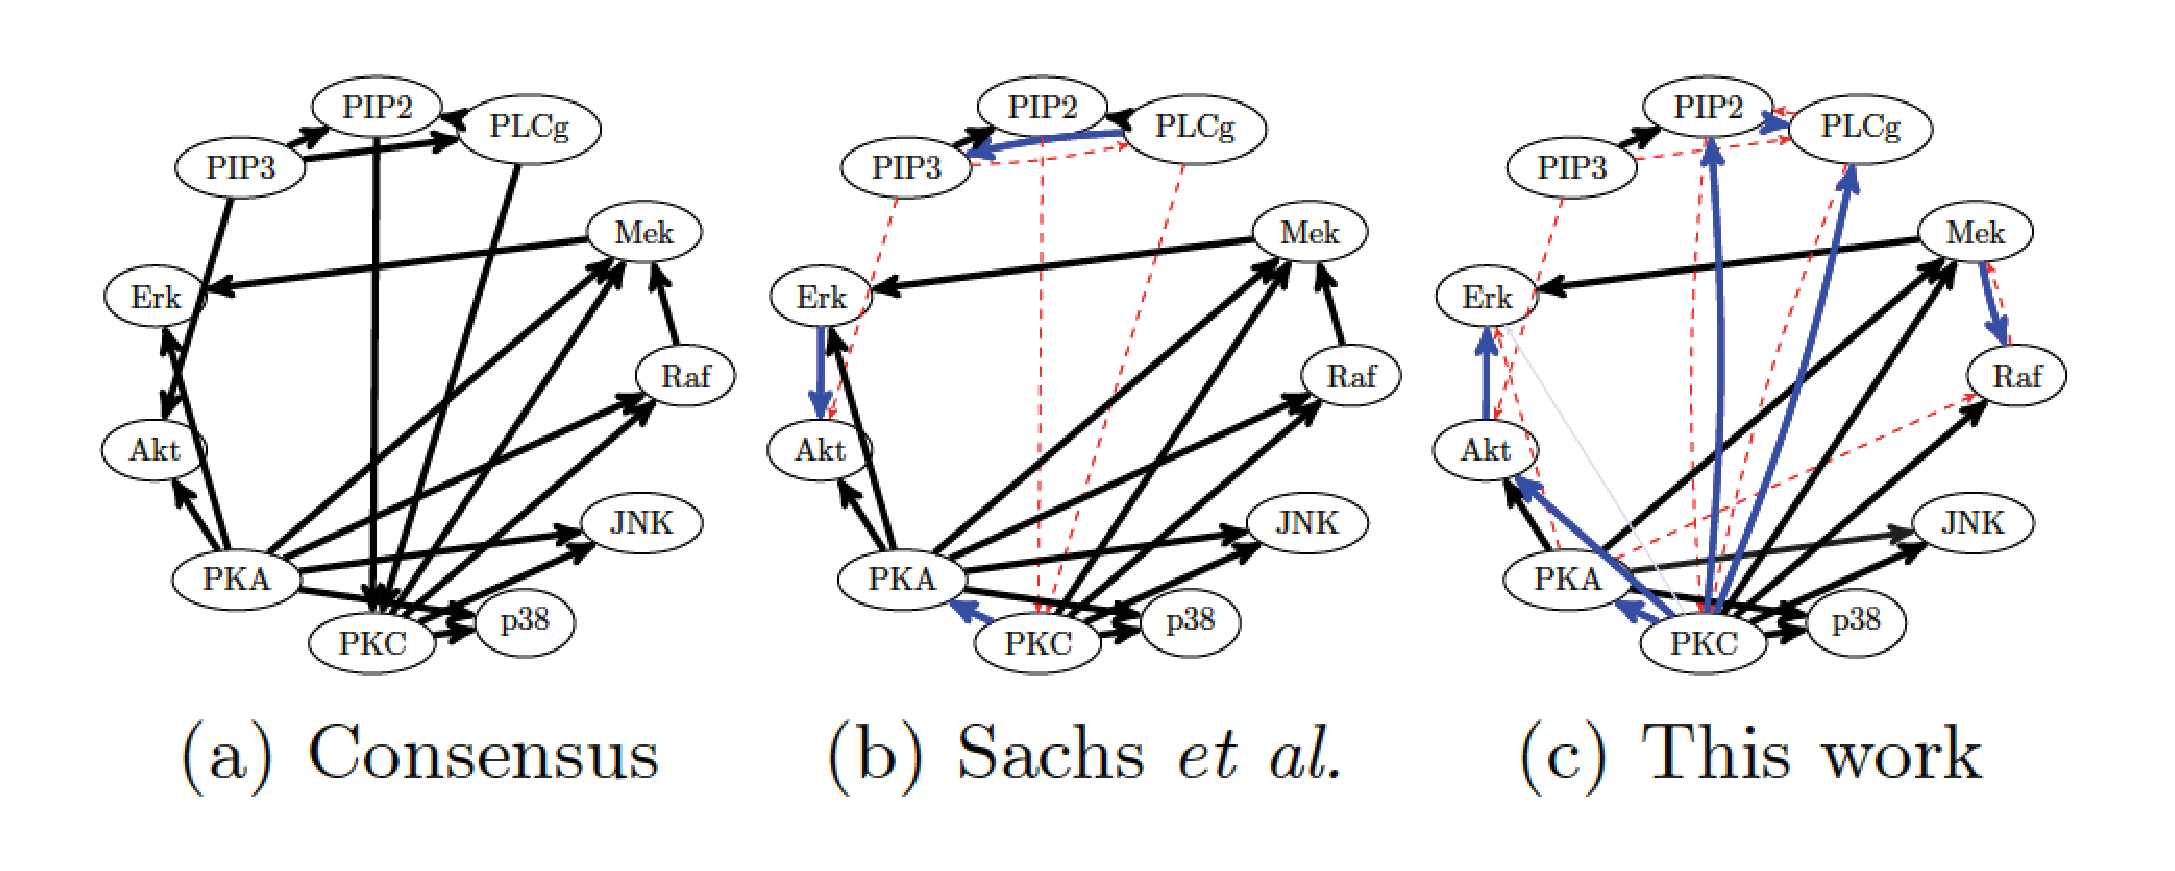
\includegraphics[width=1.1\linewidth]{img/dummy_sachs.eps} 
\caption{{\bf[DUMMY FIGURE]} Our results compared with the consensus network on the T-cell dataset.}
\label{fig:sachs}
\end{figure}


\section{Discussion}

\appendix
\section{Unsupervised Multitask Learning to Interpret Independence Tests}
We want the SparsityBoost term in the scoring function to emphasize the cases where there is strong evidence that an edge should not be present (i.e. conditional independence), while effectively disregarding cases with evidence of dependence between pairs of variables.  This is because we do not search over all possible conditioning sets, and hence just because we have evidence that $X_i$ and $X_j$ are dependent for a particular conditioning set does not prove that edge $E_{ij} \in G^*$.  Hence we define the SparsityBoost term for edge $E_{ij}$ and conditioning set C to be $$sb(E_{ij} | C; D) = -\log(P(H_1)),$$ where $H_1$ is the alternative hypothesis of dependence.  This satisfies our requirements, since when $P(H_0)$ is large, $sb$ is large, and vice versa.  In an attempt to avoid confusion, we will use a lower-case p to denote 

Note that it is not straightforward to use an independence test to claim with confidence that $H_0$ is true.  Any test with a null hypothesis of independendence allows one to reject the independence model with some degree of confidence given a small enough p-value, but on the other hand, a large p-value does not mean that one can be confident that the model is actually independent.  For example, a large p-value could just mean that the test is underpowered to detect any alternative models.  To address this, we follow \cite{efron2004large} and compute $p(H_0)$ as follows.

Suppose that we perform m conditional independence tests with null hypotheses $H_0^1, H_0^2, \ldots, H_0^m$, giving the statistics $T_1, T_2, \ldots, T_m$ and corresponding p-values, $P_1, P_2, \ldots P_m$, where $P_i = P(T_i \geq t_i | H_0^i)$.  Then under the null hypothesis, $H_0^i$, it is well known that $P_i$ follows a uniform distribution over [0, 1], whereas under the alternative hypothesis $H_1^i$, $P_i$ will tend to 0 as the amount of data increases.  Hence we can use the fact that we are performing many conditional independence tests to construct an empirical distribution over the resulting p-values, and then further represent this distribution as a mixture over $H_0$ and $H_1$, i.e. $$f(p) = f_0(p)p_0 + f_1(p)(1 - p_0).$$  The distributions of p-values are generated by considering all pairs of variables in the network conditioned on all possible sets of size k, for k up to some maximum size (here we use 2).  We fit separate distributions for each k, since larger conditioning sets correspond generally to a decrease in the power of the statistical test.  We let $f_0$ be uniform\footnote{It turns out that, due to the fact that we are computing the p-value from the KCI test using some approximations, namely matching the first two moments of the asymptotic null distribution to a Gamma distribution, the p-values corresponding to independence are not perfectly uniform, but rather are shifted towards 0, a phenomenon mentioned in \cite{zhang2012kernel}.  This leads to an underestimate of $p_0$, which corresponds to a conservative SparsityBoost term.  We argue that this is acceptable, since qualitatively speaking, Type II errors (falsely accepting the null hypothesis) are more detrimental to the score than Type I errors (falsely rejecting the null hypothesis).}, as theory predicts, and for $f_1$ we use a mixture of a tall, narrow uniform distribution near 0, and an exponential\footnote{In cases where we have many very small p-values, if we don't use the narrow uniform distribution near 0 and only fit an exponential for $f_1$, the small p-values dominate the fit, leading to an overly-steep exponential.}.  Hence we have $$f(p) = p_0\mathds{1}_{[0 \leq p \leq 1]} + (1 - p_0)\left( a \lambda e^{-\lambda p} + (1 - a) \mathds{1}_{[p \leq \delta]}\dfrac{1}{\delta} \right) $$  This distribution has four parameters, which we fit using the following procedure: \begin{enumerate} \item By assuming that no p-values corresponding to dependence lie in the range [0.5, 1], we estimate p0 using the formula: $$\widehat{p_0} = \dfrac{2 \times ( \# \text{ of p-vals} \in [0.5, 1])}{\text{total \# of p-vals}}$$  To make this more robust, we perform 200 bootstrap resamples of the data, and our final estimate is the average of the $p_0$ estimates from each of these bootstrap samples. \item We use MLE to fit the three remaining parameters, $\lambda, \delta$, and $a$, simultaneously. \item For each p-value, we compute the probability of dependence using Bayes' rule: $$P(H_1) = f_1(p)*(1 - p_0) / f(p).$$ \end{enumerate}  

Figure \ref{cite:pvals} shows an example of the result of this procedure.  These results were generated using 200 data points sampled from the child network structure using the quadratic gaussian model described above.  The top row shows the distribution of p-values resulting from applying the KCI test, along with our fit of $f(p)$ and the individual components, $f_0(p)p_0$ and $f_1(p)(1 - p_0)$.  The bottom row shows the resulting functions for $P(H_1).$  As stated above, the SparsityBoost score for each test, $sb(X_i, X_j|C; D)$ is then computed as $-\log P(H_1)$.  Notice that going from left to right in the bottom row, the functions become more shallow, consistent with the decrease in power when conditioning on more variables.

\begin{figure}[h]
\centering
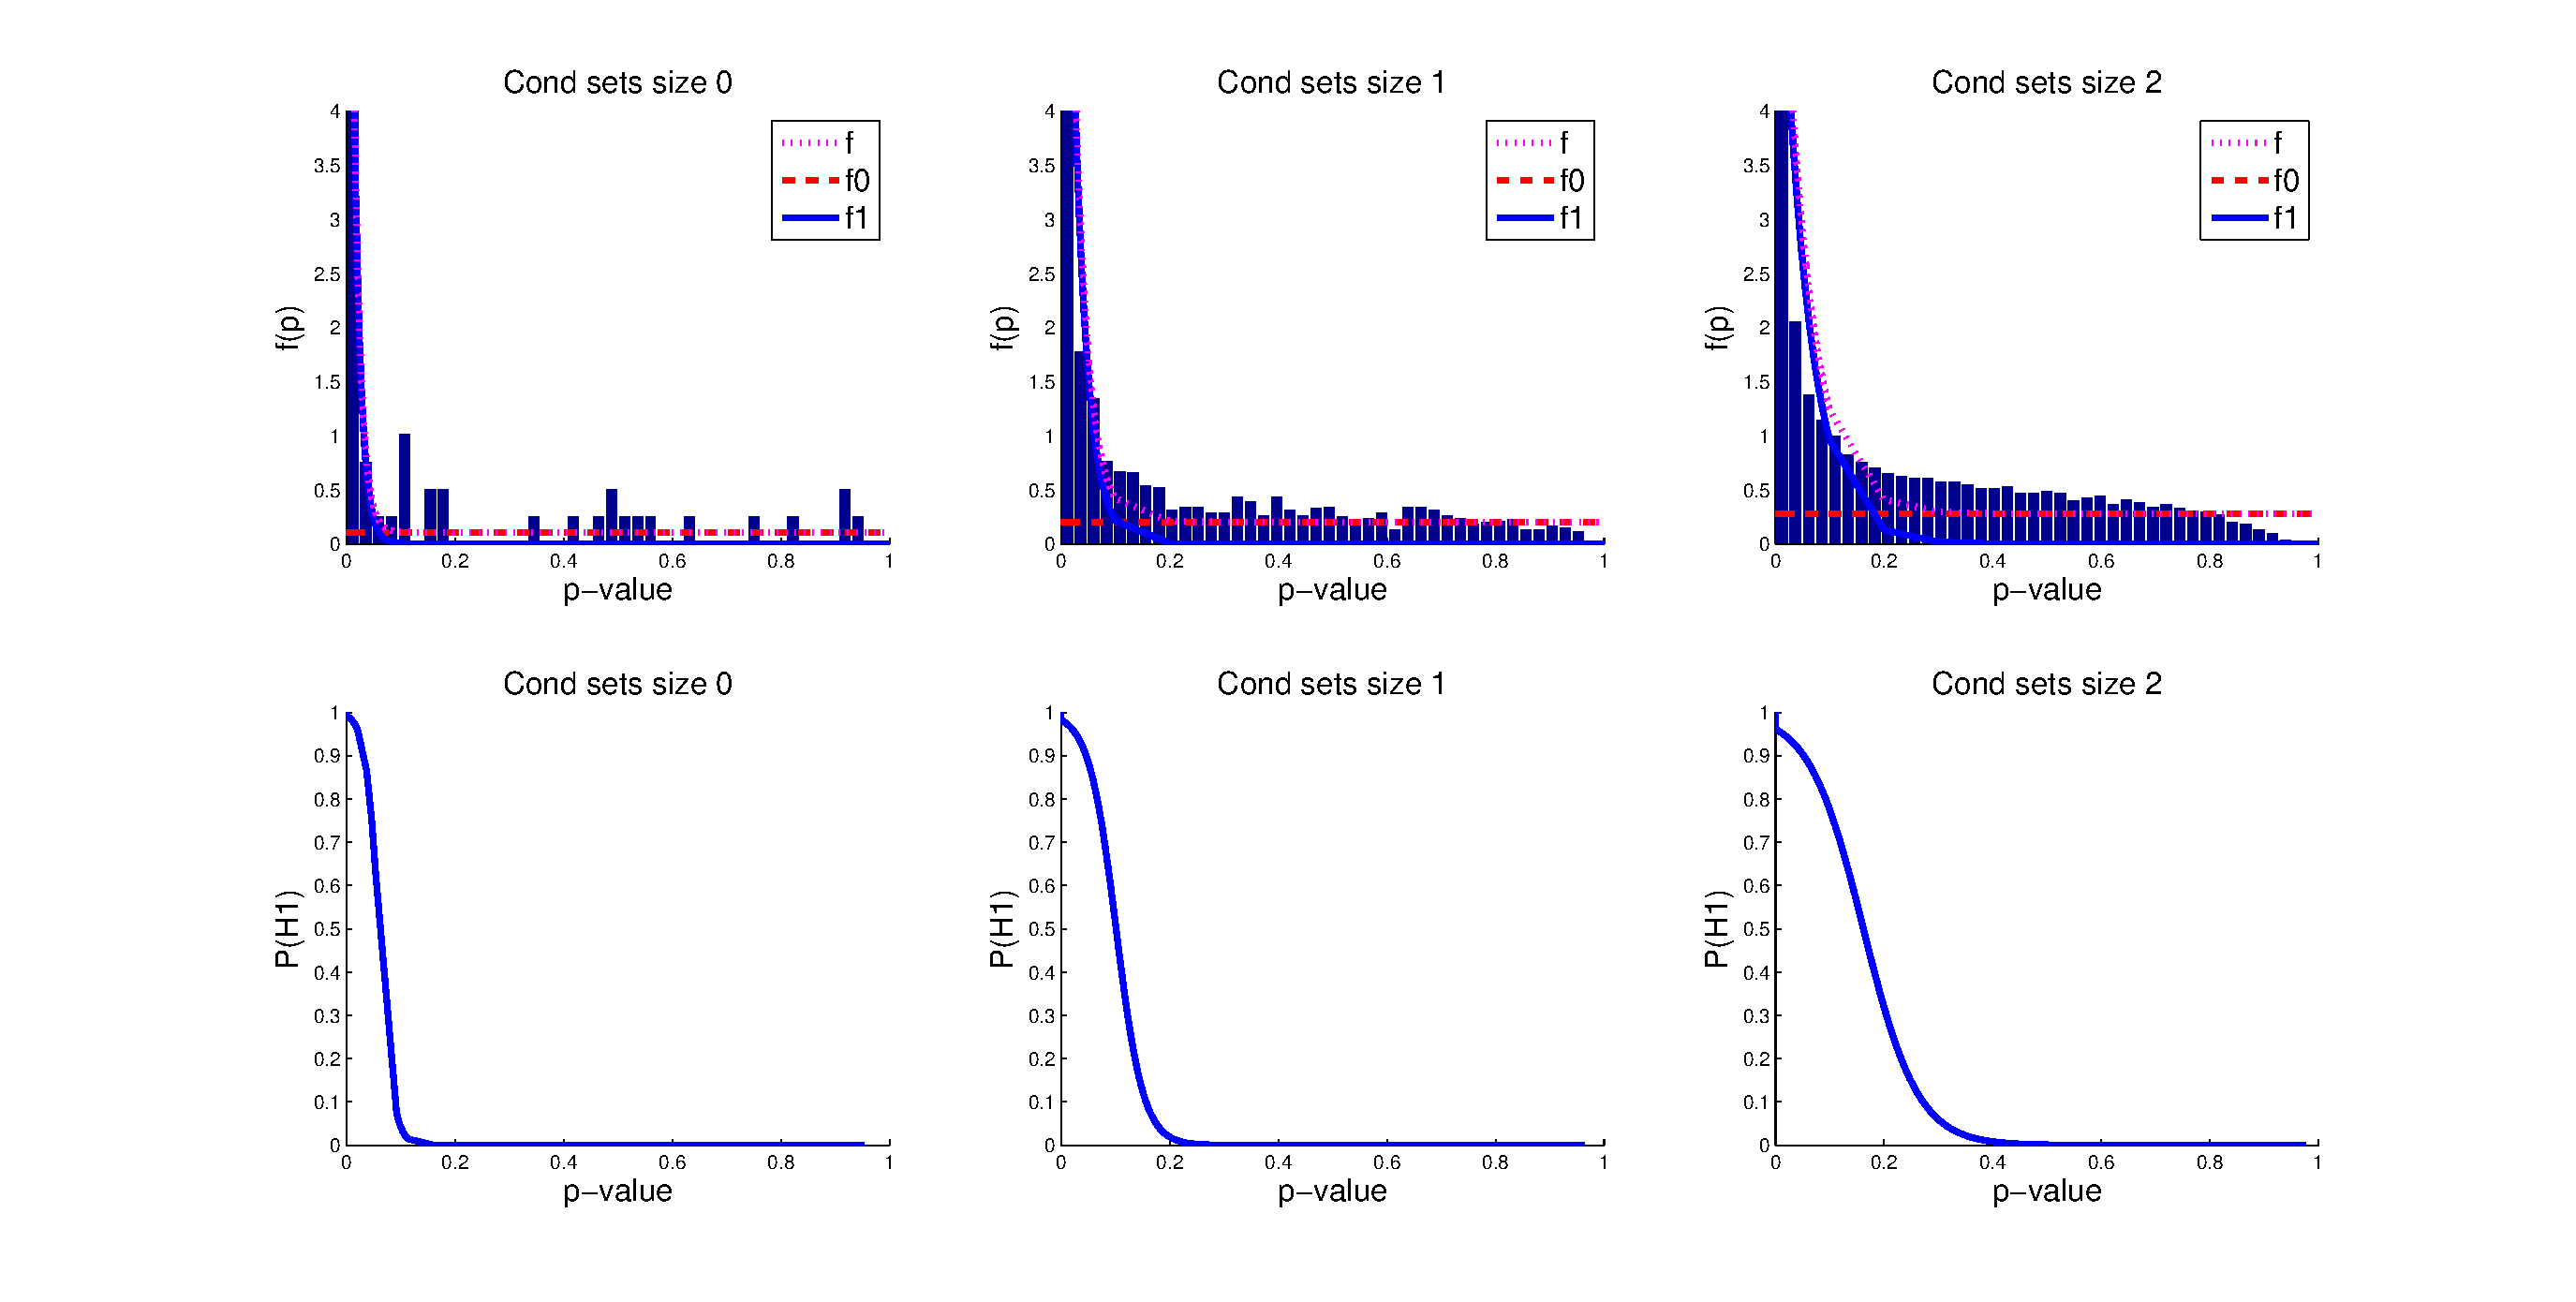
\includegraphics[width=1\linewidth]{img/child_200_pval_fits.eps}
\caption{Example of result of our procedure for computing $P(H_1)$, using 200 data points sampled from the child network structure, using the quadratic gaussian model described above. The top row show the distribution of KCI p-values, along with our fit of $f(p)$ and the individual components, $f_0 \cdot p_0$ and $f_1 \cdot (1 - p_0)$.  The bottom row shows the resulting functions for $P(H_1).$}
\label{fig:pvals}
\end{figure}


\include{appendix}

\begin{small}
%\renewcommand\bibname{References}
\bibliographystyle{abbrvnat}
%\bibliographystyle{authordate1}
%\bibliographystyle{amsnomr}
\bibliography{bibliography}
\end{small}



\end{document}
